\documentclass[10pt,letterpaper]{article}
\usepackage[margin=0.88in,top=0.78in,bottom=0.82in]{geometry}
\usepackage[T1]{fontenc}
\usepackage{newtxtext,newtxmath}
\usepackage{microtype}
\usepackage{amsmath}
\usepackage{booktabs,tabularx,array,multirow}
\usepackage{graphicx}
\usepackage{xcolor}
\usepackage{tikz}
\usetikzlibrary{arrows.meta,positioning,fit,calc,shapes.geometric}
\usepackage{enumitem}
\usepackage{titlesec}
\usepackage{caption}
\usepackage{hyperref}
\usepackage{fancyhdr}
\usepackage{float}

\definecolor{econblue}{RGB}{20,55,95}
\definecolor{slate}{RGB}{78,88,104}
\definecolor{mist}{RGB}{242,245,249}
\definecolor{lightblue}{RGB}{226,237,248}
\definecolor{lightgold}{RGB}{250,243,224}
\definecolor{lightgreen}{RGB}{231,244,237}
\definecolor{rulegray}{RGB}{200,207,216}
\definecolor{danger}{RGB}{145,60,55}
\hypersetup{colorlinks=true,linkcolor=econblue,citecolor=econblue,urlcolor=econblue,
 pdftitle={Synthetic Cultural Agents from Aggregate Anchors},
 pdfauthor={Augusto Gonzalez-Bonorino, Kseniia Biriukova, Monica Capra}}
\setlength{\parindent}{1.1em}
\setlength{\parskip}{0.16em}
\setlength{\headheight}{17pt}
\titlespacing*{\section}{0pt}{1.0em}{0.28em}
\titlespacing*{\subsection}{0pt}{0.65em}{0.2em}
\titleformat{\section}{\large\bfseries\color{econblue}}{\thesection.}{0.5em}{}
\titleformat{\subsection}{\normalsize\bfseries\color{econblue}}{\thesubsection}{0.45em}{}
\setlist[itemize]{leftmargin=1.3em,itemsep=0.08em,topsep=0.12em}
\captionsetup{font=small,labelfont={bf,color=econblue},skip=4pt}
\pagestyle{fancy}
\fancyhf{}
\fancyhead[L]{\small\color{slate} EconLLM Lab \textperiodcentered\ Synthetic Cultural Agents}
\fancyhead[R]{\small\color{slate}\thepage}
\renewcommand{\headrulewidth}{0.35pt}
\renewcommand{\headrule}{\hbox to\headwidth{\color{rulegray}\leaders\hrule height \headrulewidth\hfill}}

\newcommand{\E}{\mathbb{E}}
\newcommand{\Pcal}{\mathcal{P}}
\newcommand{\Gcal}{\mathcal{G}}
\newcommand{\Acal}{\mathcal{A}}
\newcommand{\Dcal}{\mathcal{D}}
\newcommand{\WVS}{\textsc{wvs}}
\newcommand{\GPS}{\textsc{gps}}
\newcommand{\DPO}{\textsc{dpo}}
\newcommand{\LLM}{\textsc{llm}}
\newcommand{\SCA}{\textsc{sca}}

\begin{document}
\thispagestyle{empty}
\begin{center}
\vspace*{0.65cm}
{\color{econblue}\rule{\textwidth}{1.1pt}}\\[0.45em]
{\LARGE\bfseries\color{econblue} Synthetic Cultural Agents from Aggregate Anchors}\\[0.22em]
{\large\bfseries A Falsifiable Protocol for Constructing Population-Level Choice Policies}\\[0.42em]
{\small\itshape ``Population-level'' denotes the source of the anchor, not an estimated human response distribution.}\\[0.25em]
{\color{econblue}\rule{\textwidth}{0.5pt}}\\[0.7em]
{\large Augusto Gonzalez-Bonorino\textsuperscript{1} \quad Kseniia Biriukova\textsuperscript{2} \quad Monica Capra\textsuperscript{1,3}}\\[0.42em]
{\small \textsuperscript{1}EconLLM Lab and Arizona State University \quad
\textsuperscript{2}Arizona State University \quad
\textsuperscript{3}Claremont Graduate University}\\[0.55em]
{\normalsize Working paper \textperiodcentered\ August 2026}
\end{center}

\vspace{0.45em}
\noindent\colorbox{mist}{\parbox{0.965\textwidth}{\small\vspace{0.25em}
\textbf{Status of this version.} This is a methods-first working-paper draft. Its conceptual protocol, proposed rejection design, and scope boundary are stated as commitments. The multi-country experiment, placebo controls, and pipeline-sensitivity results are intentionally represented by \emph{predeclared planned} result shells rather than invented findings; this draft is not a public preregistration. A verified USA/Mexico pilot is retained only as an Appendix diagnostic.\vspace{0.25em}}}

\section*{Abstract}
Social scientists increasingly use language models to simulate survey respondents or to align models with named communities. Both approaches obscure a central question: what exactly enters the model, and what evidence would justify interpreting its output as population-relevant? We propose a constructive alternative. A researcher declares an \emph{aggregate anchor}---a vector of population-level measurements---and freezes a protocol that maps the anchor into synthetic pairwise data and then into a language-model choice policy. Country or identity labels are absent from primary inference prompts. The resulting object is therefore not an imitation of an identified person or group, nor an estimated population response distribution; it is an aggregate-anchor-induced synthetic choice policy. Its scientific value is empirical, not assumed. We specify five testable links: anchor transmission, policy encoding, anchor relevance relative to permuted-anchor placebos, external transport to independent human survey distributions, and sensitivity to upstream generation choices. We implement the protocol with country-level Global Preference Survey anchors, synthetic preference pairs, and Direct Preference Optimization, and state a planned World Values Survey analysis with non-LLM, base-model, cultural-prompt, and placebo baselines. The paper contributes a transparent way to construct and potentially reject synthetic cultural policies while drawing a sharp boundary around claims it cannot support: individual representation, full preference-distribution recovery, and downstream causal or structural inference.

\noindent\textbf{Keywords:} synthetic cultural agents; aggregate anchors; language models; preference optimization; survey simulation; falsification; culture

\section{A construction problem, not an impersonation problem}
Language models are now routinely asked to stand in for people: a prompt supplies a demographic profile, a country name, or a social identity, and the model is asked to answer a survey ``as'' that person or population. This practice is attractive because it is cheap and scalable. It is also scientifically precarious. Prompted synthetic respondents can be highly sensitive to wording and model version, and their distributions can differ materially from human survey distributions \cite{argyle2023,bisbee2024}. More fundamentally, an inference-time persona makes it difficult to distinguish information supplied by the researcher from stereotypes or associations retrieved by the model.

The alternative is not to claim that a model has discovered a culture. It is to construct a model object from declared population-level information and then submit that construction to tests that can fail. We call the resulting object an \emph{aggregate-anchor-induced synthetic choice policy}. The policy is built from a country-level preference profile, but it is not asserted to represent any individual in that country. This boundary matters: evidence that models can flatten or misportray identity groups is a warning against treating synthetic outputs as voices of the people they purport to emulate \cite{wang2025}.

Our contribution is a protocol, not a theorem of human-preference recovery. A protocol specifies: which aggregate measurements enter; how they are rendered; how scenarios, response pairs, labels, and quality filters are generated; how the policy is estimated; and which internal, placebo, external, and sensitivity tests decide whether the construction is useful. The protocol is constructive because it creates a policy under researcher-authored rules. It is falsifiable because each link in the construction makes a separate empirical commitment.

The first implementation uses the Global Preferences Survey (\GPS), which reports country-level profiles for trust, risk taking, patience, altruism, and positive and negative reciprocity \cite{falk2018}. These anchors yield synthetic preference pairs; Direct Preference Optimization (\DPO) fits lightweight country-specific adapters relative to a common base policy \cite{rafailov2023}. The planned primary external criterion is a theory-mapped battery of World Values Survey (\WVS) item distributions. Crucially, country information is excluded from the primary evaluation prompt. This removes a direct country-token channel; it does not prove that all country-associated information is absent from base-model knowledge, scenario wording, or the profile. Thus the relevant question is not whether a model can retrieve a country label at inference. It is whether a policy induced by a declared aggregate anchor has externally useful behavior under a transparent, fixed procedure.

This paper makes four contributions: a formal statement of the aggregate-anchor construction problem and its scientific object; a modular protocol with anti-leakage, provenance, and reproducibility requirements; an empirically testable design built on five links---anchor transmission, policy encoding, anchor relevance, external transport, and operator robustness; and a predeclared multi-country comparison of the constructed policy against base-model, country-prompt, non-LLM, and permuted-anchor baselines, whose results are deliberately not pre-judged here.

\section{Positioning: where this protocol differs}
The closest literatures differ in both their information source and the location at which that information enters the model. Early ``silicon sample'' work conditions models on detailed respondent profiles and asks whether generated responses resemble human samples \cite{argyle2023}. Subsequent evidence finds instability, distributional mismatch, and inferential risks in such replacement exercises \cite{bisbee2024}. A second family fine-tunes models on human preference or survey-response data. These approaches may be appropriate when individual records or empirical response distributions are available; their claim is correspondingly closer to learned human response behavior. A third family evaluates or aligns models against named cultural communities.

\begin{table}[H]
\centering\small
\caption{Four approaches to LLM behavior associated with social-science targets. The final row is this paper's object.}\label{tab:positioning}
\begin{tabularx}{\textwidth}{@{}p{2.45cm}p{2.3cm}p{2cm}X@{}}
\toprule
\textbf{Approach} & \textbf{Training information} & \textbf{Conditioning locus} & \textbf{Central claim}\\
\midrule
Persona prompting & identity or demographic profile & inference prompt & model imitates a named respondent/group\\
Microdata fine-tuning & individual responses or distributions & weights and/or prompt & model learns observed response behavior\\
Cultural alignment & named community preferences or norms & weights and/or prompt & model aligns to an identified target\\
\textbf{Aggregate-anchor SCA} & synthetic pairs induced by declared aggregate measurements & weights; no country prompt in primary evaluation & a protocol-induced policy has passed stated tests of transport and robustness\\
\bottomrule
\end{tabularx}
\end{table}

The protocol uses familiar computational components but makes no novelty claim for them. A language model provides conditional probabilities over candidate responses; \DPO{} provides a tractable way to fit a policy from pairwise preferences; low-rank adaptation makes separate adapters practical \cite{rafailov2023,hu2022,dettmers2023}. Our contribution is to specify how aggregate measurements enter the synthetic-data operator and how the resulting policy is subjected to tests that distinguish construction success from merely plausible prose.

\section{The scientific object and its boundary}
\subsection{Aggregate anchors}
For country $c$, let
\begin{equation}
z_c=(z_{c1},\ldots,z_{cK})\in\mathbb{R}^K
\label{eq:anchor}
\end{equation}
be a vector of pre-existing population-level measurements selected before training. In the first implementation, $K=6$ and $z_c$ contains \GPS{} country scores, represented in the pipeline as standardized deviations from global means. An aggregate anchor is an input to a construction procedure. It is \emph{not} an individual record, a country name shown at inference, or a moment condition automatically satisfied by a trained policy.

We call such an input a \emph{declared} anchor: it is chosen by the researcher from a pre-existing, citable measurement source under a written inclusion rule, and it is fixed before training and before any outcome is inspected. A declared anchor is thus a researcher-committed input, whereas an \emph{identified} anchor is one recovered from the data.

\subsection{A frozen construction protocol}
We define a protocol as
\begin{equation}
\Pcal=(Z,R,G,S,Q,A,E),
\label{eq:protocol}
\end{equation}
where $Z$ records the anchor source and country frame; $R$ is the deterministic anchor-to-profile rendering rule; $G$ is the scenario, response-pair, and label-generation procedure; $S$ is scoring, quality control, and filtering; $Q$ records prompts and direct-token anti-leakage restrictions; $A$ is the policy estimator and its training configuration; and $E$ is the planned evaluation, placebo, and sensitivity design. Conditional on an archived run manifest, the model-mediated stages of $G$ and $S$ are stochastic realizations; the protocol is not equivalent to a deterministic mapping from $z_c$ to data. In the implemented protocol, $Z$ is the GPS ingestion and country frame of Section~6.1, $R$ the deterministic profile renderer, and $G$ the teacher, generator, and selector stages of Section~4.2. $S$ is the scorer and the quality-control gates, $Q$ the frozen prompts, $A$ the DPO fit of Section~4.3, and $E$ the tests of Section~5.

Given a reference policy $\pi_{\mathrm{ref}}$, the protocol generates a country-specific synthetic dataset $\Dcal_c=\Gcal_{\Pcal}(z_c)$ and fits
\begin{equation}
\widehat\pi_c^{\Pcal}=\Acal\!\left(\Dcal_c;\pi_{\mathrm{ref}}\right).
\label{eq:policy}
\end{equation}
Equation \eqref{eq:policy} defines a conditional distribution over candidate responses induced by a declared anchor and a frozen protocol. It does \emph{not} assert $\widehat\pi_c^{\Pcal}=P_{\mathrm{human},c}$, where $P_{\mathrm{human},c}$ denotes a human response distribution. That equality is an empirical transport hypothesis, not a definitional fact.

\subsection{What this construction does not identify}
Country averages do not identify which individuals hold which preferences, how preferences co-vary with demographic characteristics, or the full within-country distribution. The protocol therefore does not claim to recover individual heterogeneity, subgroup distributions, or a country's latent culture. Nor does it license reduced-form causal estimation, structural parameter recovery, or policy counterfactuals without a separate measurement and identification argument. These are not rhetorical caveats; they determine the object of study.

\begin{figure}[H]
\centering
\begin{tikzpicture}[>=Latex, node distance=6mm and 7mm, every node/.style={font=\footnotesize,align=center},
 box/.style={draw=econblue, rounded corners=2pt, thick, minimum height=10mm, text width=28mm, fill=lightblue},
 test/.style={draw=slate, rounded corners=2pt, thick, minimum height=9mm, text width=30mm, fill=lightgold},
 resultbox/.style={draw=green!50!black, rounded corners=2pt, thick, minimum height=10mm, text width=31mm, fill=lightgreen}]
\node[box] (z) {Declared aggregate anchor\\$z_c$};
\node[box, right=of z] (g) {Frozen synthetic-data operator\\$R,G,S,Q$};
\node[box, right=of g] (a) {DPO estimator\\$A$};
\node[resultbox, right=of a] (pi) {Synthetic choice policy\\$\widehat\pi_c^{\Pcal}$};
\node[test, below=12mm of g] (internal) {Internal tests\\anchor transmission; policy encoding};
\node[test, below=12mm of pi] (external) {External tests\\placebo; transport; operator robustness};
\draw[->,thick] (z)--(g);
\draw[->,thick] (g)--(a);
\draw[->,thick] (a)--(pi);
\draw[->,thick,dashed] (g)--(internal);
\draw[->,thick,dashed] (pi)--(external);
\draw[->,thick,dashed] (internal)--node[below,font=\scriptsize]{failure revises or rejects protocol}(external);
\end{tikzpicture}
\caption{The paper's scientific object. Solid arrows construct a policy. Dashed arrows are tests, not guarantees. A failed test rejects a claim about this protocol; it does not prove that a population lacks the relevant preference.}\label{fig:object}
\end{figure}

\section{From anchors to synthetic choice policies}
\subsection{Anti-leakage and profile rendering}
The primary implementation begins with the \GPS{} vector and renders it into an anonymized quantitative profile. The rendering states the magnitude and direction of each standardized score without inserting a country name. In the primary evaluation prompt, country and demographic labels are likewise omitted. This direct-token anti-leakage design does not establish cultural validity or prove that country-associated information is absent. It establishes a narrower, auditable fact: any difference between adapters cannot be attributed to country tokens in the primary inference prompt. The claim must be complemented by audits of scenario text, profile re-identifiability, and whether a classifier can infer country from generated artifacts.

\subsection{Synthetic data operator}
The operator proceeds through five conceptually distinct stages. A teacher model first proposes behaviorally distinct facets and culturally neutral scenarios for each preference dimension, and a generator then creates two plausible, opposing responses to each fixed scenario while holding non-target traits constant. An anchor-aware selector chooses the response aligned with the country profile; an independent scorer assigns both responses scores on all six dimensions; and deterministic quality-control rules retain a pair only when the scorer reports adequate target separation and acceptable directional consistency.

\noindent\textbf{Example (illustrative).} Suppose Mexico's patience z-score is $+0.32$, and the rendering stage translates it into the anonymized profile text ``standardized patience score moderately above the reference mean, with a correspondingly low temporal-discounting tendency.'' The teacher then proposes a culturally neutral scenario---a respondent deciding between an immediate small reward and a delayed larger one---and the generator fixes two opposing responses: A opts for the immediate reward, B waits for the larger one, with the instructions holding risk attitudes and income constraints constant. The anchor-aware selector, consulting the profile's positive sign, retains B for Mexico. The independent scorer assigns both responses six-dimension scores: B shows adequate separation on patience, while both remain close on the five non-target dimensions. The deterministic quality-control rules then admit the A/B pair, since target separation exceeds the threshold and the direction is consistent with the positive z-score. This trace illustrates the pipeline mechanics; it is not an empirical result.

\begin{figure}[H]
\centering
\begin{tikzpicture}[>=Latex, node distance=4mm and 6mm, every node/.style={font=\scriptsize,align=center},
 data/.style={draw=econblue, rounded corners=2pt, thick, minimum height=8mm, text width=24mm, fill=lightblue},
 model/.style={draw=slate, rounded corners=2pt, thick, minimum height=8mm, text width=25mm, fill=mist},
 gate/.style={draw=danger, rounded corners=2pt, thick, minimum height=8mm, text width=23mm, fill=lightgold}]
\node[data] (gps) {GPS vector\\$z_c$};
\node[data, right=of gps] (render) {Deterministic\\profile rendering};
\node[model, right=of render] (teacher) {Teacher: facets\\and scenarios};
\node[model, right=of teacher] (pair) {Generator: fixed\\opposing pairs};
\node[model, below=of pair] (selector) {Selector: country-\\specific pair label};
\node[model, left=of selector] (scorer) {Scorer: six-\\dimension scores};
\node[gate, left=of scorer] (qc) {Deterministic QC\\and contamination gate};
\node[data, left=of qc] (dpo) {Country DPO\\training set};
\draw[->,thick] (gps)--(render)--(teacher)--(pair);
\draw[->,thick] (pair)--(selector);
\draw[->,thick] (render.south)|-(selector.west);
\draw[->,thick] (selector)--(scorer);
\draw[->,thick] (scorer)--(qc)--(dpo);
\end{tikzpicture}
\caption{Current implementation architecture. The profile rendering is deterministic; the teacher, pair generator, selector, and scorer are separable model-mediated stages. The scientific-design appendix audits these choices and motivates ablations.}\label{fig:pipeline}
\end{figure}

This decomposition matters. Calling every upstream choice ``teacher bias'' obscures the actual sources of dependence: scenario construction, response-pair generation, country-specific selection, scorer judgments, and filter thresholds may each change the synthetic training distribution. The empirical design therefore treats the full operator as an object of sensitivity analysis.

\subsection{Policy estimation}
For synthetic triplets $(x,y_w,y_\ell)\in\Dcal_c$, \DPO{} fits a policy relative to $\pi_{\mathrm{ref}}$ by minimizing
\begin{equation}
\mathcal{L}_{\mathrm{DPO}}(\pi)= -\E_{(x,y_w,y_\ell)\sim\Dcal_c}\left[\log\sigma\!\left(\beta\log\frac{\pi(y_w\mid x)}{\pi_{\mathrm{ref}}(y_w\mid x)}-\beta\log\frac{\pi(y_\ell\mid x)}{\pi_{\mathrm{ref}}(y_\ell\mid x)}\right)\right].
\label{eq:dpo}
\end{equation}
\DPO{} is a pairwise-preference estimator with reference-policy regularization \cite{rafailov2023}. Here it fits synthetic preferences generated by $\Pcal$. It is not a constrained estimator that mechanically enforces $\E[f(Y)]=z_c$, and we make no such claim.

\section{Making the construction empirically rejectable}
The phrase ``falsifiable'' is useful only if it names propositions, estimands, and failure consequences. This working-paper version supplies the test architecture, but not a public timestamped registration or final numerical thresholds; it should therefore be read as a proposed rejection design. Before any scaled outcome is inspected, the archived analysis plan will fix the unit of analysis, primary metric, comparison, practical margin, randomization/materialization count, uncertainty procedure, and country/domain/protocol decision rule for every row in Table~\ref{tab:tests}. Each test concerns a distinct link; passing one does not imply passing another.

\begin{table}[H]
\centering\small
\caption{The five rejection points of an aggregate-anchor construction.}\label{tab:tests}
\begin{tabularx}{\textwidth}{@{}p{2.45cm}p{3.2cm}X@{}}
\toprule
\textbf{Claim} & \textbf{Predeclared evidence} & \textbf{Interpretation of failure}\\
\midrule
Anchor transmission & label/sign agreement, target separation, QC rates, anchor swaps & the synthetic operator does not express the declared input reliably\\
Policy encoding & held-out synthetic-pair recovery; policy-distance stability & DPO does not retain the contrast present in the synthetic data\\
Anchor relevance & real-anchor versus permuted-anchor placebo adapters & apparent gains may reflect generic synthetic tuning rather than anchor information\\
External transport & independent human survey distributions versus base, prompt, and non-LLM baselines & this protocol does not generalize to the chosen external criterion\\
Operator robustness & scenario, generator, selector, scorer/QC, materialized-data, and training-seed ablations & the conclusion depends on arbitrary or unstable upstream choices\\
\bottomrule
\end{tabularx}
\end{table}

\subsection{Internal tests: transmission and encoding}
Anchor transmission asks whether changing $z_c$ changes labels and retained pairs in the direction dictated by the declared rule. It is assessed with country-by-dimension label summaries, quality-control pass rates, target-versus-nontarget separation, contamination ratios, and anchor-swap diagnostics. The current implementation makes an especially important test available: because the selector is instructed to implement a sign rule, the primary sensitivity comparison must contrast a deterministic sign-labeling operator with the legacy LLM selector. Policy encoding asks whether the trained adapter reproduces held-out synthetic contrasts and whether independently trained policies are stable under repeated materializations of the same protocol.

\subsection{Anchor relevance: a restricted permutation distribution}
A central negative control draws many restricted permutations of country anchors before synthetic generation while retaining all other stages. The final plan will predeclare any strata used to preserve region, sample availability, or anchor magnitude, and will evaluate the real-anchor statistic in its resulting empirical null distribution. Each placebo uses the same data volume, model family, and training budget as the reference protocol. If real-anchor adapters do not outperform this distribution on predeclared external outcomes, the data do not support the claim that aggregate anchors add useful information beyond generic synthetic fine-tuning.

\subsection{External transport and uncertainty}
External transport is a predictive-criterion claim: the policy's induced option probabilities improve alignment with independently collected human response distributions. It is neither recovery nor validation of a complete country distribution. For a question $q$ with valid options $\mathcal{Y}_q$, let $\ell_{\widehat\pi_c}(y\mid q)$ denote the total log probability assigned to the token sequence encoding answer option $y$ under a fixed prompt and option-order rule. The policy yields
\begin{equation}
\widehat P_c(y\mid q)=\frac{\exp\{\ell_{\widehat\pi_c}(y\mid q)\}}{\sum_{j\in\mathcal{Y}_q}\exp\{\ell_{\widehat\pi_c}(j\mid q)\}},
\label{eq:choiceprob}
\end{equation}
and the primary descriptive discrepancy is total variation distance,
\begin{equation}
\mathrm{TVD}(\widehat P_c,P_c)=\frac{1}{2}\sum_{y\in\mathcal{Y}_q}|\widehat P_c(y\mid q)-P_c(y\mid q)|.
\label{eq:tvd}
\end{equation}
For each country--item cell, $P_c$ is the survey-weighted empirical option distribution after a frozen harmonization map for option wording, order, invalid outputs, and Likert categories. The analysis will report absolute TVD and paired differences from every baseline, together with practical margins. It will distinguish finite-survey sampling uncertainty, country and item aggregation, materialized synthetic datasets, and DPO training seeds; a hierarchical or randomization-based aggregation rule will be fixed before outcome inspection. A bootstrap over survey items is useful only as a robustness calculation for the declared item battery---not as respondent sampling uncertainty, an item-universe inference, or uncertainty about an upstream model-mediated pipeline.

\section{Empirical implementation: predeclared design}
\subsection{Data roles and country frame}
The first implementation uses \GPS{} as the anchor source and \WVS{} Wave 7 as the primary independent outcome surface. Before a scaled run, the authors will archive an immutable country inclusion/exclusion rule, a named 10--15-country panel from the \GPS{}$\times$\WVS{} intersection, and a frozen theory-led item battery. The battery must separately list construct-linked confirmatory outcomes---with an expected direction or distributional relation for each \GPS{} dimension---and descriptive/exploratory outcomes. The existing 35-item pilot map contains 30 mapped items and five demographics; it is not itself the confirmatory map for the scaled study.

AmericasBarometer and the Integrated Values Surveys may serve as secondary instrument or temporal replications if multi-country overlap is adequate. World Bank indicators are contextual covariates for exploratory heterogeneity analysis, not direct choice-distribution criteria.

\subsection{Anchor sources: criteria, GPS, and alternatives}

A source must satisfy a small set of conditions before it can anchor the construction. It must be pre-existing and citable, fixing the reference in the public record rather than constructing it for this study; it must offer population-level aggregates rather than individual microdata, because the outcome surface is itself country-level; and it must be theoretically linked to the constructs of interest while remaining independent of the evaluation surface, so that anchoring on \WVS{} country means while evaluating \WVS{} items would be circular. It must also offer broad country coverage and valid, comparable measurement across countries.

\GPS{} is a defensible first implementation of these criteria. Its country scores are aggregates by construction, derived from measures of six economic preferences that were validated ex ante in incentivized experiments, collected in representative samples across 76 countries---a set that overlaps the \WVS{} Wave 7 country frame. The data are public and citable, and the criteria are fixed before any scaled run.

Alternatives exist if the criteria recommend them: \WVS{}/EVS country means, with the caveat of overlap with typical evaluation surfaces; Schwartz value country scores (PVQ/ESS); Hofstede dimensions; Inglehart--Welzel cultural-map coordinates; and the GLOBE project. Table~\ref{tab:anchor-sources} lists these candidates with their principal caveats. The method is agnostic to the specific source, so long as the criteria above hold.

\begin{table}[H]
\centering
\small
\caption{Candidate anchor sources and their principal caveats.}
\label{tab:anchor-sources}
\begin{tabularx}{\textwidth}{@{}l X l@{}}
\hline
Source & What it measures & Key caveat \\
\hline
\GPS{} & Six economic preferences (trust, risk-taking, patience, altruism, positive and negative reciprocity) & Aggregate by construction; experimentally validated \\
\WVS{}/EVS means & Country-level value orientations and attitudes & Circular when the evaluation surface is \WVS{} itself \\
Schwartz (PVQ/ESS) & Ten basic human values at country level & Fewer countries; values are not preference measures \\
Hofstede dimensions & Work-related cultural dimensions & Dated samples; dimensions are not preference measures \\
Inglehart--Welzel map & Emancipative and secular value coordinates & Two-dimensional reduction of a larger item space \\
GLOBE & Societal practices and leadership values & Organizational focus; limited item overlap \\
\hline
\end{tabularx}
\end{table}

\subsection{Baselines and primary comparison}
Every country is evaluated against four mandatory baselines: (i) the unmodified base model; (ii) a country-named cultural-prompt baseline; (iii) a named non-LLM aggregate benchmark fixed before outcome inspection; and (iv) the restricted permuted-anchor distribution. The country prompt is deliberately included despite violating direct-token anti-leakage because it answers a distinct practical question: whether an explicit persona retrieves useful information more effectively than the constructed policy. The analysis must report provenance-sensitive construction success separately from predictive alignment; a cultural prompt may be practically predictive while failing the former objective.

The primary cross-country claim will compare each fixed policy to each country's human distribution. Under unconditioned prompts, this is \emph{fixed-policy proximity}, not evidence that the model conditions on a country at inference. Country-level permutation tests and cross-country patterns become informative only with more than two adapters. The design will report gains and failures, rather than defining success as a uniformly positive average.

\subsection{Operator-sensitivity panel}
A stratified 4--6-country subset is run before the full panel. The reference protocol is compared with alternative scenario banks, alternate pair-generation materializations, deterministic-sign versus legacy-selector labels, QC-threshold variations, a scorer-diagnostic-only/no-QC arm where feasible, restricted anchor permutations, and repeated DPO seeds. Each arm reports effects on (i) synthetic-data diagnostics, (ii) learned-policy stability, and (iii) external transport. At least three independently materialized scenario/pair banks are retained per condition. The full panel proceeds only if this subset establishes adequate anchor transmission, excludes obvious high-contamination pairs under a predeclared rule, and rejects the basic placebo explanation.

\section{Planned reporting structure}
\noindent\colorbox{mist}{\parbox{0.965\textwidth}{\small\textbf{Status.} This section contains the planned reporting logic and table shells. It will be completed only from frozen artifacts produced under the protocol in Section 6. No scaled empirical outcome is claimed in this draft.}}

\subsection{Anchor transmission and synthetic-data quality}
Table \ref{tab:resultshell} will report country-by-dimension label agreement, QC retention, target separation, and contamination. Failure is informative: a low pass rate, directional reversal, or high cross-dimension contamination is evidence against the operator, not a reason to selectively discard countries.

\subsection{Policy encoding and repeatability}
The next report will separate held-out synthetic-pair recovery from repeated-run policy stability. A policy that perfectly fits a single synthetic dataset but varies strongly across regenerated datasets has not demonstrated a stable aggregate-anchor construction.

\subsection{External transport, placebo, and failure cases}
The primary table will compare reference adapters, base models, cultural prompts, non-LLM benchmarks, and permuted-anchor adapters. Results will be disaggregated by country and preference domain. A negative or null country is a result: it narrows the scope of the protocol rather than being silently pooled away.

\begin{table}[H]
\centering\small
\caption{Predeclared main result shell. Values are filled only after the frozen multi-country experiment.}\label{tab:resultshell}
\begin{tabularx}{\textwidth}{@{}p{2cm}p{2.15cm}p{2.2cm}p{2.2cm}X@{}}
\toprule
\textbf{Country} & \textbf{Protocol arm} & \textbf{Synthetic diagnostics} & \textbf{External discrepancy} & \textbf{Interpretation}\\
\midrule
$c_1$ & real anchor & [pending] & [pending] & [pending]\\
$c_1$ & permuted-anchor placebo & [pending] & [pending] & anchor relevance test\\
$c_1$ & country-prompt baseline & [pending] & [pending] & practical comparator\\
$\vdots$ & $\vdots$ & $\vdots$ & $\vdots$ & $\vdots$\\
\bottomrule
\end{tabularx}
\end{table}

\section{Discussion}
The protocol changes the question posed to synthetic cultural agents. It does not ask whether an \LLM{} can speak for a country, nor does it assume that country-level averages identify individual preferences. It asks whether a declared aggregate profile can be transformed into a reproducible policy whose synthetic provenance is visible and whose external relevance is testable.

This distinction has practical consequences. The method may be useful for exploratory measurement, hypothesis generation, survey-item design, and benchmark construction when its tests support those applications. It is not a substitute for collecting human data, and it should not be used to infer individual beliefs, to represent subgroups, or to support causal and structural claims without additional evidence. The correct scientific outcome is sometimes rejection: an anchor may fail to transmit, an adapter may fail to encode, a placebo may perform similarly, or an external criterion may not transport.

The protocol also makes clear why operator sensitivity is substantive. If a finding disappears when a scenario bank, selector, quality-control threshold, or training materialization changes, then the finding belongs to a fragile synthetic pipeline rather than to the aggregate anchor. Conversely, stability across those choices does not prove representation, but it increases confidence that the observed policy behavior is an attribute of the specified construction rather than an incidental artifact.

\section*{Code and data availability}
The SCA2 implementation, frozen evaluation artifacts, and this working-paper source are available at \url{https://github.com/EconLLM-Lab/SCA2_PofW}. A claim-ready release will identify an immutable repository tag/commit, code license, model/API versions, and an artifact manifest. \GPS{} data are documented by Falk et al. \cite{falk2018}; \WVS{} Wave 7 data and documentation are available from the World Values Survey Association under DOI \url{https://doi.org/10.14281/18241.18} \cite{wvs2022}. Raw survey microdata are not redistributed with the repository.

\newpage
\appendix
\section{USA/Mexico pilot: a proof-of-concept diagnostic, not evidence of specificity}
The existing two-country pilot is retained because it clarifies a design boundary. Under the primary unconditioned prompt, the same model emits identical option probabilities when scored against USA and Mexico; only the external target distribution differs. Thus a matched-versus-cross comparison measures which adapter's \emph{fixed} output distribution lies closer to each population's observed responses. It does not show that the adapter knows or conditions on its target country at inference.

In the committed pilot, the Mexico adapter has mean TVD $0.4882$ on Mexico versus $0.5211$ for the base model, while the USA adapter has $0.6377$ on Mexico. The corresponding mean matched-minus-cross TVD difference is $0.1495$ with a question-resampling 95\% interval $[0.0964,0.2152]$ across 35 items. On USA outcomes, however, the Mexico adapter is approximately neutral relative to base ($0.3888$ versus $0.3958$), while the USA adapter degrades ($0.5258$). These values are verified transcriptions of the committed evaluation summaries.

The pilot therefore does not establish country specificity. A single fixed adapter can dominate another fixed adapter against either country, and $C=2$ cannot reveal a stable country-by-policy cross-over pattern. The item bootstrap quantifies sensitivity to this 35-item battery, not uncertainty from training runs, model generation, respondents, or country sampling. The pilot motivates---rather than substitutes for---the multi-country placebo and operator-sensitivity design in the main paper.

\section{Adversarial scientific-design audit of the synthetic-generation pipeline}
\label{app:audit}
\noindent\colorbox{lightgold}{\parbox{0.965\textwidth}{\small\textbf{Scope and evidence.} This independent appendix is a static audit of the specified pipeline and its tests, not an empirical validation of generated records. The targeted test suite was attempted but could not be collected in the review environments because \texttt{pandas}/\texttt{numpy} dependencies were unavailable. The inspected tests predominantly mock model completions (for example, \texttt{synthetic\_generation/tests/test\_generate.py:139--184} and \texttt{test\_score.py:13--182}); no test-pass, psychometric-validity, inter-rater-reliability, or model-stability claim follows from this audit.}}

\subsection{Blocker findings}
\textbf{Replace the LLM selector with a deterministic sign rule for non-zero target scores.} The selector is explicitly instructed that positive $z$ implies A and negative $z$ implies B, while fixed A/B responses were already generated as positive/negative target loadings (\texttt{generate.py:170--180, 237--279}). It is therefore a stochastic, prompt-mediated implementation of a supplied deterministic label rather than an independent estimator of country-specific preference. It introduces label noise, permits irrelevant use of the other five profile dimensions, and depends on mutable model behavior. The primary construction should use A when $z>0$ and B when $z<0$, with $|z|$ near zero excluded, flagged, or handled under a separately justified probabilistic rule. The current exact-zero fallback is internally inconsistent: selector guidance asks for the ``less extreme'' option whereas QC treats zero as positive (\texttt{generate.py:250--255; score.py:204--206}).

\textbf{Treat LLM scoring/QC as process diagnostics, not a validity screen.} The scorer receives the target dimension and rubric, scores the already selected chosen/rejected texts, and QC retains rows whose scorer-derived target difference agrees with the known \GPS{} sign (\texttt{score.py:46--64, 119--130, 204--235}). This is a second model confirming a target specified by design, not an independent measurement of cultural preferences or construct validity. No calibration against blinded human annotations, reliability analysis, held-out behavior, or threshold justification is present in the inspected code/tests. The scores may be useful operational diagnostics, but should not be described as validating a population-level construct.

\subsection{Major findings}
\textbf{Selection-on-the-outcome and unfiltered contamination threaten validity.} Scoring follows country-specific selection, so fixed A/B pairs are repeatedly scored in country-oriented order rather than once blind to country and choice (\texttt{generate.py:429--474; score.py:119--146}). Cross-dimension movement is calculated but does not determine \texttt{qc\_status}; export removes only non-pass statuses, so high-contamination pairs can remain (\texttt{score.py:209--221; export.py:323--329}). The recommended design scores canonical A/B options once under blinded target and option order, orients scores arithmetically after deterministic labeling, reports all cross-loading distributions, and either predeclares a contamination gate or treats contamination as descriptive only.

\textbf{Prompts attempt control but do not demonstrate it.} The pair generator is instructed to vary only the target trait while holding the other five constant (\texttt{generate.py:175--180}); this is an instruction, not evidence of compliance. Optional curated anchors are injected into scenario and triplet prompts (\texttt{generate.py:72--76, 156--160}), creating a provenance channel that must be versioned and separated from evaluation materials. Country names are absent from profile text (\texttt{profiles.py:44--65}), a useful safeguard, but all six numeric dispositions remain available to selection (\texttt{generate.py:263--275}).

\textbf{Generation reproducibility is incomplete.} The manifest records config snapshots, \GPS{} vectors, costs, scenario counts, timestamp, and a short Git hash; export shuffling uses a seed (\texttt{export.py:41--50, 367--399}). However, the pipeline seed is not passed to model calls and teacher/generator temperatures are non-zero (\texttt{config.py:225--228; generate.py:41--49, 194--202}). Manifests lack input hashes, resolved model revisions, dependency locks, raw-checkpoint hashes, prompts, and repository dirty state. Resume can reload current input data before rescoring an old checkpoint (\texttt{run.py:363--418}). Outputs should therefore be treated as dated stochastic realizations until immutable input and full-run provenance are archived.

\subsection{Efficiency-preserving changes and a minimal ablation}
Deterministic signs eliminate all per-country selector calls. The default 120 fixed triplets (six dimensions times 20 scenarios) otherwise generate 120 times the number of countries selection calls. Score each canonical pair once rather than once per country, orient scores locally by country sign, and compute QC arithmetic locally; this reduces country-linear scorer calls and removes country/choice-order leakage. Facets and scenarios are already batched, but per-triplet selector reasoning payloads are not used for labeling or QC and can be omitted or sampled for audit, while preserving raw responses and request metadata for remaining calls.

The minimum ablation uses a fixed scenario/A--B bank and compares: (i) deterministic signs versus legacy LLM selection; (ii) no QC versus scorer diagnostic-only versus scorer plus a predeclared contamination exclusion; and (iii) anchors off versus on. Each condition should retain at least three independently generated banks, stratified by dimension and $z$-score magnitude. Report label disagreement with the deterministic rule, QC retention, cross-loading distributions, blinded human ratings of target loading/non-target leakage/plausibility/option balance, and the full range of downstream conclusions. If legacy-selector and deterministic-sign estimates differ materially, the former is an unvalidated alternative rather than the primary dataset.

\section{Training configuration}
\label{app:trainconfig}
The reference training configuration in Table~\ref{tab:trainconfig} is fixed before any scaled run; every adapter in the pilot and scaled protocol is estimated against it, and any deviation from it is declared as a sensitivity arm rather than an ad hoc adjustment. Entries are transcribed from and verified against the canonical training artifacts under \texttt{DPO\_train\_test/}.

\begin{table}[H]
\centering\small
\caption{Reference training configuration for the country-specific DPO adapters. All variants in the operator-sensitivity panel are declared relative to this configuration.}\label{tab:trainconfig}
\begin{tabularx}{\textwidth}{@{}p{3.6cm}Xp{4cm}@{}}
\toprule
\textbf{Component} & \textbf{Setting} & \textbf{Source/status}\\
\midrule
Base model & Llama-3.1-8B-Instruct (\texttt{meta-llama/Llama-3.1-8B-Instruct}) & \texttt{DPO\_train.ipynb}\\
QLoRA quantization & 4-bit NF4, double quant, fp16 compute & \texttt{DPO\_train.ipynb}\\
LoRA rank/alpha & $r=16$, $\alpha=32$, dropout $0.05$ & \texttt{DPO\_train.ipynb}\\
LoRA target modules & \texttt{q\_proj}, \texttt{k\_proj}, \texttt{v\_proj}, \texttt{o\_proj} (attention projections) & \texttt{DPO\_train.ipynb}\\
DPO beta & $\beta=0.1$ & \texttt{DPO\_train.ipynb}\\
Learning rate/schedule & $1\times10^{-4}$, cosine, warmup ratio $0.03$ & \texttt{DPO\_train.ipynb}\\
Epochs & 1 & \texttt{DPO\_train.ipynb}\\
Batch size/gradient accumulation & per-device batch 1; 16 accumulation steps (effective 16) & \texttt{DPO\_train.ipynb}\\
Synthetic triplets per country & $\approx$3{,}594 generated per country; 2{,}875 in the training split (80/20, seed 42) & \texttt{DPO\_train.ipynb}\\
Hardware & Single Colab-class GPU (Tesla T4 in the committed run) & \texttt{DPO\_train.ipynb}, \texttt{README.md}\\
\bottomrule
\end{tabularx}
\end{table}

\section{Protocol artifacts required for a claim-ready version}
A claim-ready version will archive: (i) country inclusion rules; (ii) anchor and item-map versions; (iii) prompts, temperatures, model IDs, and endpoint versions; (iv) raw scenario, pair, selection, and scoring outputs; (v) QC tables; (vi) training manifests and adapter hashes; (vii) evaluation outputs; and (viii) analysis code for item, country, generation, and training-seed uncertainty. A remote API seed is not itself a sufficient reproducibility guarantee; materialized datasets are the primary artifacts.

\begin{thebibliography}{99}
\bibitem{argyle2023}
L.~P. Argyle, E.~C. Busby, N.~Fulda, J.~R. Gubler, C.~Rytting, and D.~Wingate.
\newblock Out of one, many: Using language models to simulate human samples.
\newblock \emph{Political Analysis}, 31(3):337--351, 2023.

\bibitem{bisbee2024}
J.~Bisbee, J.~D. Clinton, C.~Dorff, B.~Kenkel, and J.~M. Larson.
\newblock Synthetic replacements for human survey data? The perils of large language models.
\newblock \emph{Political Analysis}, 32(4):401--416, 2024.

\bibitem{dettmers2023}
T.~Dettmers, A.~Pagnoni, A.~Holtzman, and L.~Zettlemoyer.
\newblock QLoRA: Efficient finetuning of quantized LLMs.
\newblock In \emph{Advances in Neural Information Processing Systems}, 36, 2023.

\bibitem{falk2018}
A.~Falk, A.~Becker, T.~Dohmen, B.~Enke, D.~Huffman, and U.~Sunde.
\newblock Global evidence on economic preferences.
\newblock \emph{Quarterly Journal of Economics}, 133(4):1645--1692, 2018.

\bibitem{hu2022}
E.~J. Hu, Y.~Shen, P.~Wallis, Z.~Allen-Zhu, Y.~Li, S.~Wang, L.~Wang, and W.~Chen.
\newblock LoRA: Low-rank adaptation of large language models.
\newblock In \emph{International Conference on Learning Representations}, 2022.

\bibitem{rafailov2023}
R.~Rafailov, A.~Sharma, E.~Mitchell, S.~Ermon, C.~D. Manning, and C.~Finn.
\newblock Direct preference optimization: Your language model is secretly a reward model.
\newblock In \emph{Advances in Neural Information Processing Systems}, 36, 2023.

\bibitem{wang2025}
A.~Wang, J.~Morgenstern, and J.~P. Dickerson.
\newblock Large language models that replace human participants can harmfully misportray and flatten identity groups.
\newblock \emph{Nature Machine Intelligence}, 7:400--411, 2025.

\bibitem{wvs2022}
World Values Survey Association.
\newblock World Values Survey Wave 7 (2017--2022).
\newblock DOI: \url{https://doi.org/10.14281/18241.18}, 2022.
\end{thebibliography}
\end{document}
